\chapter{Prérequis}
\label{chap:preliminaires}

Ce chapitre a pour ambition de rappeler les bases nécessaires pour la théorie de la réécriture,
des automates d'arbres, et présentera le cadre de la vérification de modèles symoblique auquel
nous nous intéresserons dans cette thèse. Pour plus détails, le lecteur pourra trouver plus d'informations
sur la réécriture dans~\cite{BaaderN-book98} et dans~\cite{TATA} pour les automates d'arbres.


\section{Termes et réécriture}

\begin{definition}
  Une \textbf{signature} $\F$ est un ensemble de symboles de fonctions dont l'arité est fixée par
  une fonction $\phi : \F \rw \N$. Par $\F_i$, on distingue l'ensemble des symboles $ f \in \F$
  d'arité $\phi(f) = i$. Dès lors, $\F_0$ caractérise l'ensemble des \textbf{constantes}.
\end{definition}


\begin{definition}
  Soit $\F = \{ f_2, g_1, h_2, \dots\}$ une signature\footnote{\footnotesize Pour définir rapidement $\F$, Chaque symbole est indicé par son arité}.
  Soit $\X$ un ensemble de \textbf{variables} tel que $\X \cap \F = \emptyset$.
  L'ensemble $\TFX$ dénote l'\textbf{algèbre de termes} engendrée par la signature $\F$ à partir de $\X$. On définit $\TFX$ comme le plus petit ensemble
  tel que:
  \begin{itemize}
  \item $\X \subseteq \TFX$ 
  \item pour tout $n \in \N$ et $f \in \F_n$, si $t_1, \dots, t_n \in \TFX$ alors $f(t_1, \dots, t_n) \in \TFX$
  \end{itemize}
\end{definition}
Les éléments de $\TFX$ sont appelés des \textbf{termes}. On note $\TF$, l'algèbre des \textbf{termes clos} -- \textit{i.e.} 
sans variable -- lorsque $\TFX$ est engendrée à partit de $\X = \emptyset$.
Cette définition inductive nous indique que toute variable est un terme, 
et que l'application d'un symbole de fonction à des termes engendre de nouveaux termes. Cette construction permet de voir
les termes comme des arbres étiquetés.
Considérons $\F = \{ f_3, g_2, h_1 \}$ et $\X = \{x, y, z\}$. On peut alors construire le terme $f(g(x,h(y)), g(x, g(y, z)), h(x))$
que l'on peut représenter par l'arbre de la figure~\ref{fig:terme-arbre}.

\begin{figure}[ht!]
  \centering
  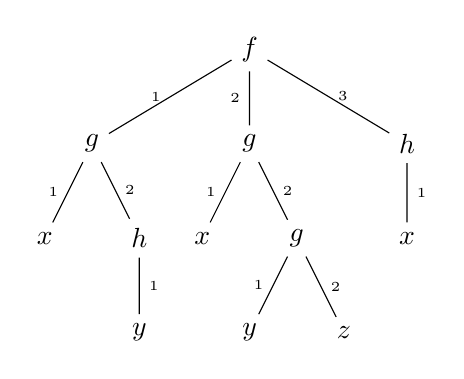
\begin{tikzpicture}[level distance=12mm]
    \tikzstyle{level 1}=[sibling distance=20mm]
    \tikzstyle{level 2}=[sibling distance=12mm]
    \node{$f$}%[grow=right]
    child{node{$g$}
      child{node{$x$}
        edge from parent node[left] {\tiny $1$}
      }
      child{node{$h$}
        child{node{$y$} edge from parent node[right] {\tiny $1$}}
        edge from parent node[right] {\tiny $2$}
      }
      edge from parent node[left] {\tiny $1$}
    }
    child{node{$g$}
      child{node{$x$}
        edge from parent node[left] {\tiny $1$}
      }
      child{
        node{$g$}
        child{node{$y$} edge from parent node[left] {\tiny $1$}}
        child{node{$z$} edge from parent node[right] {\tiny $2$}}
        edge from parent node[right] {\tiny $2$}
      }
      edge from parent node[left] {\tiny $2$}
    }
    child{node{$h$}
      child{node{$x$} edge from parent node[right] {\tiny $1$}}
      edge from parent node[right] {\tiny $3$}
    };
  \end{tikzpicture}
  \caption{\footnotesize le terme $f(g(x,h(y)), g(x, g(y, z)), h(x))$ vu comme un arbre étiqueté}
  \label{fig:terme-arbre}
\end{figure}

La représentation d'un terme sous forme d'arbre permet de voir
facilement que le terme $f(g(x,h(y)), g(x, g(y, z)), h(x))$ est constitué des \textbf{sous-termes}
représentés par les sous-arbres dans la figure~\ref{fig:terme-arbre}.
Ainsi $g(x, g(y, z))$ est un sous-terme de $f(g(x,h(y)), g(x, g(y, z)), h(x))$.
Un sous-terme sont caractérisé par sa position à partir de la racine du terme
qui le contient. Une \textbf{position} $p$ est définie comme un \textbf{mot de $\NN$} qui correspond
à un chemin dans l'arbre. Le mot vide $\epsilon$ correspond à la racine du terme.

\begin{definition}
  Soit un terme $t \in \TFX$. L'ensemble $\pos(t)$ des positions de $t$ se définit inductivement
  comme:
  \begin{itemize}
  \item $\pos(t)= \{ \epsilon\} $ si $t \in \X$
  \item $\pos(f(t_1,\dots,t_n)) = \{ \epsilon \} \cup \{i.p \mid 1 \leq i \leq n
    \et p \in \pos(t_i) \}$
  \end{itemize}
\end{definition}


Si $p \in \pos(t)$, alors $t|_p$ dénote le \textbf{sous-terme de} $t$ \textbf{à la position} $p$ et
$t[s]_p$ dénote le terme obtenu après le \textbf{remplacement} du sous-terme $t|_p$ par le terme $s$.
On peut les définir par induction sur $p \in \pos(t)$:
\begin{itemize}
\item $t|_\epsilon = t$
\item $f(t_1,\dots, t_n)[s]_{i.p} = t_i|_p$
\end{itemize}
et
\begin{itemize}
\item $t[s]_\epsilon = s$
\item $f(t_1,\dots, t_n)[s]_{i.p} = f(t_1,\dots, t_i[s]_p,\dots,t_n)$
\end{itemize}

\begin{definition}
  L'ensemble des variables d'un terme $t \in \TFX$ est dénoté par $\vars(t)$ et se définit simplement
  comme $\vars(t) = \{ x \in \X \sep \exists p \in \pos(t) \st x = t|_p\}$
\end{definition}
On remarque pour tout terme $t \in \TFX$, $\vars(t) = \emptyset$ alors $t$ est un terme clos, ce qui est équivalent à $t \in \TF$.

\begin{definition}
  Une substitution est une fonction $\sigma$ de $\X$ vers $\TFX$, telle que 
  pour un certain nombre de variables $x \in X$ on a $x \not= \sigma(x)$.
  L'ensemble des ces variables est noté $\dom(\sigma)$.
  On étend les substitutions à des endomorphismes de $\TFX$. 
  On note alors $t\sigma$ (ou $t.\sigma$) l'application de la substitution $\sigma$ au terme $t$ 
  qui remplace toute occurence des variables par leur image respective via $\sigma$:
  \begin{itemize}
  \item $t\sigma = \sigma(t)$ lorsque $t \in \X$
  \item $f(t_1, \dots, t_n)\sigma = f(t_1\sigma, \dots, t_n\sigma)$
  \end{itemize}
\end{definition}
On appelle $id$, la substitution dont le domaine $\dom(\sigma)$ est vide.
Pour tout terme $t \in \TFX$, on a $t.id = t$.

On dit qu'un terme $t$ est une \textbf{instance} d'un terme $s$ lorsqu'il existe une substitution
$\sigma$ telle que $t = s\sigma$.

Un système de règles de réécriture -- TRS en abrégé
\footnote{\footnotesize abréviation issue de la formulation anglaise équivalente {\em term rewriting system}} -- 
$\R$ est un ensemble de règles de réécriture. 

\begin{definition}
  Une \textbf{règle de réécriture} est une paire, notée $l \rw r$, composée de deux termes $l, r \in \TFX$,
  telle que $l \not \in \X$, et $\var(l) \supseteq \var(r)$. 
  On appelle $l$ et $r$ respectivement le membre gauche et le membre droit de la règle.
  Une règle de réévriture est \textbf{linéaire à gauche} (ou à droite) si chaque variable de $\X$, 
  n'apparait pas plus d'une fois dans son membre gauche (droit {\textit resp.}).
  %Une règle est \textbf{linéaire} si elle est à la fois linéaire à gauche et à droite.
\end{definition}

Un système de règles de réécriture est linéaire à gauche (ou à droite) si chacune 
de ses règles est linéaire à gauche (à droite {\textit resp.}). De même, le système est 
linéaire si il est linéaire à gauche et à droite.

\begin{definition}
  Si $\R$ est un TRS, alors on note $\rw_{\R}$ la relation de réécriture qu'il induit sur les termes.
  On dit que le terme $s$ se réécrit en $t$ par la règle $l \rw r \in \R$ si et seulement si l'un des sous-termes de $s$
  est une instance de $l$ et $t$ est le terme $s$ où l'instance de $l$ est remplacée par l'instance de $r$ correspondante:

  \noindent $s \rw_\R t \equ$
  \begin{flushright}
    $\exists\ l \rw r \in \R,\ p \in Pos(s),\ \sigma: \X \rw \TFX \textrm{ tels que }\quad \quad \quad$
    $s|_p = l\sigma \quad \et \quad  t = s[r\sigma]_p$
  \end{flushright}
\end{definition}
Ainsi, la règle $g(x, y) \rw y$ permet de réécrire le terme $h(g(x, g(y, z)))$ 
soit en $h(g(x, z))$ ou $h(g(y, z))$, suivant que l'on choisisse de réécrire le sous-terme
à la position $1.2$ ou à la position $1$.

La clôture transitive et réflexive de $\rw_\R$ se note $\rw^*_{\R}$.
Si $A$ est un ensemble de termes clos, on définit l'ensemble des $\R$-descendants 
de $A$ comme $\desc(A) = \{t \in \TF \sep \exists s \in A \st s \rw^*_{\R} t \}$.

\begin{definition}
  Une \textbf{équation} est une paire, notée $s = t$, composée de deux termes $s, t \in \TFX$.
  Si $e$ est l'équation $s = t$, alors deux termes $u$ et $v$ sont égaux modulo $e$ si et seulement si
  
  \noindent $u =_e v \equ$\\
  \[\exists\ p \in Pos(s),\ \sigma: \X \rw \TFX \textrm{ tels que } \quad s|_p = l\sigma \quad \et \quad  t = s[r\sigma]_p\]
  
  Si $E$ est un ensemble d'équations, on note $=_E$ la plus petite relation d'équivalence qui contienne la relation
  $\{ u =_E v \sep \exists e \in E,\ u =_e v\}$
\end{definition}


\begin{definition}
  Soient $\R$ un TRS, et $E$ un ensemble d'équations. On définit la \textbf{réécriture modulo} comme la relation
  $\rw_\RE$ définie comme:
  \[\forall\ s, t \in \TFX,\quad s \rw_\RE t \equ \exists u, v \in \TFX,\quad s =_E u \rw_\R v =_E t\]
\end{definition}
De la même manière que pour $\R$, note $\rw_\RE^*$ la clôture transitive et réflexive de $\rw_\RE$, et 
on définit l'ensemble des $\RE$-descendants pour un ensemble $A$ de termes clos par
$\descE(A) = \{t \in \TF \sep \exists s \in A \st s \rw^*_{\RE} t \}$.

%\comments{Paires critiques ou pas???}
\section{Les automates d'arbres}
\label{sec:automates}

Soit $\Q$ un ensemble fini de constantes appelées \textbf{états} tel que $\Q \cap \F= \emptyset$.
On définit $\TFQ$ l'algèbre engendrée par $\F$ et $\Q$, que l'on appelle l'ensemble des \textbf{configurations}.

\begin{definition}%[Les transitions]
  \label{def:transitions}
  Dans un automate d'arbres, une \textbf{transition} est une règle de réécriture de la forme $c \rw q$, où $c$ est une configuration
  \textit{i.e.} $c \in \TFQ$ et $q \in \Q$ est un état. On distingue deux sortes de transitions dans un automate d'arbres:
  \begin{itemize}
  \item Une \textbf{transition normalisée} est une transition de la forme $f(q_1, \dots, q_n) \rw q$
    avec $f \in \F_n$, et $q_1, \ldots, q_n, q \in \Q$ sont des états
  \item Une \textbf{$\varepsilon$-transition} est une transition de la forme $q' \rw q$ où $q', q \in \Q$ sont des états
  \end{itemize}
\end{definition}

% An epsilon transition is a transition of the form $q \f q'$ where $q$ and $q'$
% are states. Any set of transition $\Delta \cup \{q \f q'\}$ can be
% equivalently replaced by $\Delta \cup \{c \f q' \sep c \f q \in \Delta \}$.

\begin{definition}% [Bottom-up nondeterministic finite tree automaton]
  Un automate d'arbres ascendant fini non-déterministe -- ou plus simplement automate d'arbres --
  pour la signature $\F$ est un quadruplet $\A= \langle \F, \Q, \Q_F,\Delta \rangle$,
  avec 
  \begin{itemize}
  \item $\Q$ un ensemble d'états,
  \item $\Q_F \subseteq \Q$ un ensemble d'états finals et,
  \item $\Delta$ un ensemble fini de transitions normalisées et de $\varepsilon$-transitions.
  \end{itemize}
\end{definition}

Un automate d'arbres $\A$ reconnaît des termes clos de $\TF$. L'exécution d'un automate d'arbres
débute en réécrivant les feuilles du terme au moyen des transitions, remplacant progressivement
chaque sous-terme par des états jusqu'à la racine du terme. La sémantique d'une exécution 
repose sur le principe qu'un terme $t$ (et donc un sous-terme) est reconnu par un certain état $q$ de l'automate lorsqu'on a
réduit $t$ en $q$ par réécriture, ce que l'on note $t \rw_\Delta^* q$ ou plus généralement $t \rw_\A^* q$. De plus, si l'état $q$
est final (\textit i.e. $q \in \Q_f$), alors $t$ est reconnu ou accepté par l'automate.

\begin{definition}
  L'ensemble des termes reconnus par l'automate $\A$ en l'état $q$ est défini par $\Lang(\A, q) = \{ t \in \TF \sep t \rw_\A^* q\}$.
  Le langage reconnu par $\A$ est $\Lang(\A) = \bigcup_{q_f\in \Q_f} \Lang(\A, q_f)$. 
\end{definition}
Sans perte de généralité, on considèrera dans la suite que \textbf{tout automate $\A$ est toujours nettoyé}
c'est à dire que $\A$ ne posssède pas d'état dont le langage est vide: $\forall q \in \Q, \Lang(\A, q) \not= \emptyset$.

\begin{example}
  Soit l'automate d'arbres $\A = \langle \F, \Q, \Q_F, \Delta \rangle$ avec
  \begin{itemize}
  \item $\F=\{et_2,v_0,f_0\}$
  \item $\Q= \{q\}$
  \item $\Q_F=\{q\}$
  \item $\Delta= \{v \rw q, et(q, q) \rw q \}$
  \end{itemize}
  Cet automate ne reconnait que les conjonctions s'évaluant à vrai (V).\\
  \begin{center}
  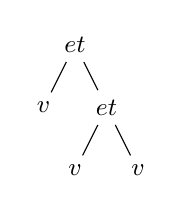
\begin{tikzpicture}[level distance=10mm, scale=.8]
    \tikzstyle{level 1}=[sibling distance=10mm]
    \tikzstyle{level 2}=[sibling distance=10mm]
    \node{\small $et$}
    child{node{\small $v$}}
    child{
      node{\small $et$}
      child{node{\small $v$}}
      child{node{\small $v$}}
    };
  \end{tikzpicture}
  $\lrw_\A$
  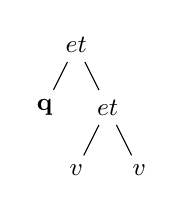
\begin{tikzpicture}[level distance=10mm, scale=.8]
    \tikzstyle{level 1}=[sibling distance=10mm]
    \tikzstyle{level 2}=[sibling distance=10mm]
    \node{\small $et$}
    child{node{\small $\mathbf q$}}
    child{
      node{\small $et$}
      child{node{\small $v$}}
      child{node{\small $v$}}
    };
  \end{tikzpicture}
  $\lrw_\A$
  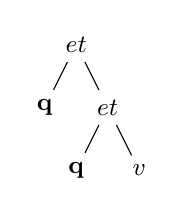
\begin{tikzpicture}[level distance=10mm, scale=.8]
    \tikzstyle{level 1}=[sibling distance=10mm]
    \tikzstyle{level 2}=[sibling distance=10mm]
    \node{\small $et$}
    child{node{\small $\mathbf q$}}
    child{
      node{\small $et$}
      child{node{\small $\mathbf q$}}
      child{node{\small $v$}}
    };
  \end{tikzpicture}
  $\lrw_\A$
  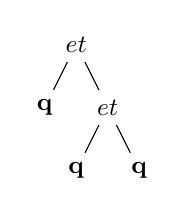
\begin{tikzpicture}[level distance=10mm, scale=.8]
    \tikzstyle{level 1}=[sibling distance=10mm]
    \tikzstyle{level 2}=[sibling distance=10mm]
    \node{\small $et$}
    child{node{\small $\mathbf q$}}
    child{
      node{\small $et$}
      child{node{\small $\mathbf q$}}
      child{node{\small $\mathbf q$}}
    };
  \end{tikzpicture}
  $\lrw_\A$
  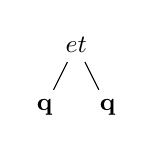
\begin{tikzpicture}[level distance=10mm, scale=.8]
    \tikzstyle{level 1}=[sibling distance=10mm]
    \tikzstyle{level 2}=[sibling distance=10mm]
    \node{\small $et$}
    child{node{\small $\mathbf q$}}
    child{node{\small $\mathbf q$}}
    ;
  \end{tikzpicture}
  $\lrw_\A$
  \begin{tikzpicture}[level distance=10mm, scale=.8]
    \tikzstyle{level 1}=[sibling distance=10mm]
    \tikzstyle{level 2}=[sibling distance=10mm]
    \node{\small $\mathbf q$};
  \end{tikzpicture}
  \end{center}

  \begin{center}
    \begin{tikzpicture}[level distance=10mm, scale=.8]
      \tikzstyle{level 1}=[sibling distance=10mm]
      \tikzstyle{level 2}=[sibling distance=10mm]
      \node{\small $et$}
      child{node{\small $v$}}
      child{node{\small $f$}}
      ;
    \end{tikzpicture}
    $\lrw_\A$
    \begin{tikzpicture}[level distance=10mm, scale=.8]
      \tikzstyle{level 1}=[sibling distance=10mm]
      \tikzstyle{level 2}=[sibling distance=10mm]
      \node{\small $et$}
      child{node{\small $q$}}
      child{node{\small $f$}}
      ;
    \end{tikzpicture}
    $\not\lrw_\A$
  \end{center}
\end{example}

\begin{property}
  \label{prop:execution}
  Soit un terme $t \in \TF $ reconnu par l'état $q \in \Q$ d'un automate $\A$. 
  On peut décomposer autant de fois que nécessaire l'exécution de l'automate pour le terme $t$.
  Tout sous-terme de $t$ est aussi reconnu par l'automate $\A$.
  \[t \rw_\A^* q \imp \forall p \in \pos(t), \exists q' \in \Q, \st t|_p \rw_\A^* q' \et t[q']_p \rw_\A^* q\]
  \includegraphics[width=12cm]{2_prerequis/automate_rev}
\end{property}


% \begin{corolary}
%   Soit une configuration $c \in \TFQ$. On définit l'ensemble des termes qui peuvent se réécire en $c$ par un automate $\A$
%   par un ensemble de substitutions de $\tau: \Q \f \TF$. Chacune des substitutions associe à chaque état $q$  un terme clos
%   $\tau(q) \in \Lang(q, \A)$ ou l'état $q$ si $\Lang(q, \A) = emptyset$,
%     Ainsi, le terme Chacune de ses fonctions
% \end{corolary}

Soit $L \subseteq \TF$ un ensemble de ensembles de termes clos. Le langage $L$ est régulier si et seulement si il existe
un automate d'arbres $\A$ tel que $L = \Lang(\A)$. Les langages réguliers de termes sont clos par union, intersection, et 
complémentation. Cependant, il est important de noter que la complémentation nécessite de déterminiser l'automate d'arbres
ce qui peut entraîner une complexité exponentielle.

\section{Le Model-Checking régulier}

Dans cette thèse, on s'intéresse à la vérification de propriétés de systèmes,
et en particulier aux systèmes pour lesquels l'ensemble des états accessibles
est infini mais peut-être modélisé de manière finie~\cite{WB98}. 
Il est à noté que l'approche envisagée fonctionne aussi 
dans le cas de systèmes à ensemble fini d'états.

Le premier problème est de fournir une représentation symbolique 
pour exprimer et manipuler des ensembles potentiellement infinis
d'états. C'est une question récurrente en vérification qui est malheureusement
indécidable, et pour laquelle il n'existe que des solutions partielles.
Ici, l'angle d'attaque retenu est celui de la vérification de modèles
à base de langage régulier de termes plus communément appelée {\em Tree Regular Model Checking
  (TRMC)}\,\cite{ALRd05}. Cette approche est une extension de l'approche qui fut initiallement introduite
pour calculer l'ensemble des états atteignables en utilisant les langages réguliers de mots~\cite{BJNT00,BLW03}.


En TRMC, on modélise un système de transitions (tel qu'un programme ou un protocole) par un triplet $(\F, I, Rel)$,
avec
\begin{itemize}
\item
$\F$ une signature permettant de construire $\TF$ l'ensemble des termes représentants les différentes configurations ou états
du système;

\item
  $I \subseteq \TF$ un ensemble régulier de configurations donc représentable par un automate d'arbres $\A$, 
  \textit{i.e.} $\Lang(\A)=I$;

\item $Rel$ est une relation de transition représentée par un ensemble de règles de réécriture
  \footnote{\footnotesize A l'origine, $Rel$ est modélisée par un transducteur d'arbres.
    Mais comme les automates d'arbres peuvent être vus comme une classe particulière de 
    systèmes règles de réécriture, on choisit ici de généraliser}.
  On impose à $\R$ d'être linéaire à gauche.
\end{itemize}

\noindent
Dans ce contexte, un programme sera alors representé par un triplet $(\F,\A,\R)$.
Ce type de modélisation est très expressif, d'une part parce que les systèmes de réécriture
linéaires à gauche sont Turing-complet~\cite{HUET-78}, et d'autre part il est facile de 
modéliser les protocoles cryptographiques~\cite{GenetK-CADE00}, ainsi que pour exprimer
un sous-ensemble important du ByteCode Java~\cite{BoichutGJL-RTA07}.
On considère le problème d'atteignabilité pour ce modèle.

\begin{definition}[Problème d'atteignabilité]
\label{def:reachability}
Soit un programme $(\F,\A,\R)$ et un ensemble $Bad$ de termes correspondant à des états
interdits que le programme ne doit jamais atteindre.
Le problème d'atteignabilité consiste à vérifier qu'il n'existe 
aucun terme de $\desc(\Lang(\A))$ qui soit dans $Bad$.
\end{definition}

Le problème d'atteignabilité permet de vérifier des propriétés de sûreté
pour le système considéré. L'ensemble $Bad$ décrit des configurations invalides 
qui ne doivent pas être atteignables pour le système.

Dans le cas d'un protocole cryptographique $Bad$ peut décrire des
configurations résultant d'une attaque du protocole ex: le message
chiffré est révélé en clair à un protagoniste externe à la
transaction\dots.

Pour les programmes Java, $Bad$ peut décrire par des états où l'on
s'apprête à accéder à une zone mémoire non définie ex: pointeur null,\dots

\section{La complétion d'automates d'arbres}
\label{sec:completion}
Dans le cas des systèmes à espace d'états fini (et de taille
raisonnable), le calcul de l'ensemble des termes atteignables
($\desc(\Lang(\A))$) peut se réduire à une simple énumération des
termes que l'on peut atteindre à partir des termes de l'ensemble
initial.  Mais il n'est pas possible d'utiliser une telle
technique sur les systèmes à espace infini d'états (ou trop
important). En effet, lorsque $\R$ ne termine pas ou si 
$\Lang(\A)$ est infini, l'ensemble $\desc(\Lang(\A))$ est
alors infini et n'est généralement pas calculable~\cite{GilleronTison-FI95}.
Dans ces cas, il est nécessaire d'\textit{accélérer} l'exploration de
l'espace d'états afin d'atteindre notamment les termes situés à une
\textit{distance infinie} des termes initiaux, pour se ramener à un 
\textit{temps de calcul} raisonnable.
C'est dans ce contexte que se place la \textbf{complétion d'automates d'arbres}
décrite dans~\cite{Genet-RTA98,FeuilladeGVTT-JAR04}.
C'est un semi-algorithme qui calcule un automate d'arbres, \textit{i.e.} une représentation
régulière (et donc finie) des ensembles infinis, qui est en général
une sur-approximation de l'ensemble des termes atteignables.
Elle peut être utilisée pour résoudre certaines instances du problème d'atteignabilité:
la complétion d'automates d'arbres est facilement paramétrable afin de définir 
la sur-approximation souhaitée~\cite{Genet-RTA98,FeuilladeGVTT-JAR04,Takai-RTA04}
pour le problème considéré.

\subsection{Principe général}

Ainsi, en utilisant l'algorithme de complétion on peut construire un
automate d'arbres $\B$ dont le langage $\Lang(\B) \supseteq
\desc(\Lang(\A))$ contient au moins tous les termes atteignables.  Il
est alors suffisant de vérifier que l'automate $\B$ ne reconnait pas
de termes de $Bad$ -- \textit{i.e.} $\Lang(\B)\cap Bad = \emptyset$ --
pour montrer que le système n'atteint jamais aucune des configurations
de $Bad$ soit $\desc(\Lang(\A))\cap Bad=\emptyset$.


% Expressivité des systèmes de réécriture :
% permettant de modéliser facilement des systèmes états/transitions,
% Outils pour assurer des vérifier des propriétés correction.
% Dans ce cadre, vérifier si un terme est atteignable ou non ?
% meme si le problème indécidable, la complétion 
% d'automates d'arbres contribue à la collection des outils capables
% de traiter le problèmes pour des ensembles de termes importants ou infinis.

% Le problème d'atteignabilité en général sous branche du  model checking (propriété de sûreté).
% transposé en réécriture et résolution du problème:
% vérifier si un terme considéré comme non-atteignable n'est effectivement pas atteignable.
% La notion d'atteignailité est toujours défini pour problème composé un ensemble initial $I$ et un système de 
% réécréture, donnés explicitement ou non.
% Discussion autour de l'exactidude du résultat de la complétion d'automates d'arbres???


% \comments{Calcul d'un ensemble régulier des termes atteignables par réécriture. 
% Cet ensemble est une surapproximation régulière (parfois exacte) de  $\R^*(I)$.

% Principe est d'utiliser les automates d'arbres comme représentation des ensembles de termes.
% Puis de réécrire des configurations de l'automate. 
% Puisqu'une configuration représente un ensemble de termes, réécriture d'une configuration de l'automate
% $\equiv$ réécrire un ensemble de termes.
% }

La complétion d'automates d'arbres termine lorsque le calcule arrive sur un point fixe,
lorsque l'automate est $\R$-clos.


\begin{definition}
  Un automate d'arbres $\B$ est dit $\R$-clos si pour tous termes $s,t$ tels que 
  $s \rw_\R t$ avec $s$ reconnu par $\B$ dans un état $q$, alors $t$ est aussi reconnu par $\B$ dans l'état $q$.
  La propriété de clôture est illustrée par le diagramme de la figure~\ref{fig:R-cloture}.
  % The situation is represented with the following graph.
  \begin{figure}[ht!]
    \centering
    $
    \xymatrix{
      s \ar[r]_{\R}\ar[d]^{*}_{\B} & t \ar@/^1.2pc/[ld]_{*}^{\B}\\
      q & %\ar[l]^{\A_{i+1}} q'
    }
    $
    \caption{\footnotesize Propriété de $\R$-clôture}
    \label{fig:R-cloture}
  \end{figure}
\end{definition}

Il est évident de constater que l'on a $\Lang(\B) \supseteq \desc(\Lang(\A))$
si $\B$ est $\R$-clos et si $\Lang(\B)\supseteq \Lang(\A)$~\cite{BoyerGJ-IJCAR08}.

D'un point de vue algorithmique, la construction d'un automate $\R$-clos, que l'on notera
$\aaex^*$, à partir de l'automate $\A$ consiste à \textit{compléter} l'automate $\A$
par de nouvelles transitions pour étendre son langage. L'algorithme de complétion
calcule une succession d'automates $\aaex^1,\aaex^2,\ldots$ en appliquant à chaque fois
l'ensemble des règles de réécriture sur $\aaex^i$ pour produire $\aaex^{i+1}$.
Le calcul peut s'arrêter lorsque l'on obtient un automate $\R$-clos 
$\aaex^k$ \textit{i.e.} tel que $\Lang(\aaex^{k+1}) \supseteq \Lang(\aaex^k)$.

\subsection{Etape de complétion : calcul exact des $\R$-descendants}


Chaque application du TRS $\R$ est appelée \textbf{étape de completion} et 
consiste à rechercher parmi les termes reconnus par l'automate qui peuvent être réécrits
dont les descendants ne sont pas encore reconnus par l'automate.
Cela revient à rechercher les \textbf{paires critiques} $\langle q, t \rangle$ 
pour lesquelles le diagramme de la figure~\ref{fig:R-cloture} n'est pas clos, \textit{i.e.}
on a $s \rw_\R t$ et $s \rw_{\A}^* q$ mais pas $t \not\rw_{\A}^* q$.

On ne considère que les paires critiques dont l'origine est localisée à la racine du terme c'est à dire
que la position $p$ à laquelle le terme est réécrit par $\R$ est $p = \epsilon$.
En effet, quelle que soit la position $p \in \pos(s)$ à laquelle on décide de réécrire le terme
$s$, on peut toujours revenir au cas d'une paire critique où la réécriture n'a lieu qu'à la racine du terme.
Il suffit de considérer l'exécution $s \rw_\A^* q$ par l'automate $\A$. 
On sait que le terme $s$ se réécrit à la position $p \in \pos(s)$ par une règle $l \rw r$ de $\R$. Ce qui signifie que le sous-terme à la 
position $p$ est une instance de $l$ donc de la forme $l\tau$, où $\tau$ est une substitution $\X \f \TF$.
Or d'après la propriété~\ref{prop:execution}, comme $s$ est reconnu par l'automate $\A$, c'est aussi le cas pour chacun de ses sous-termes
et donc en particulier il existe un état $q'$ tel que $l\tau \rw_\A^* q'$. On peut donc simplifier le problème de la paire critique $\la q, t\ra$ à la position $p$
en considérant la paire critique $\la q', r\tau\ra$ à la position $\epsilon$.


\begin{figure}[ht!]
  \centering
  \includegraphics[width=12cm]{2_prerequis/cp1}
\end{figure}
% \comments{FIGURE PAIRES CRITIQUES 1}
Ce qui revient à\\
\begin{figure}[ht!]
  \centering
  \includegraphics[width=8cm]{2_prerequis/cp2}
\end{figure}

%\comments{FIGURE PAIRES CRITIQUES 2}

% remis car il faut introduire la notation \aaex^i, utilisée dans la suite.
Une étape de complétion résout toutes les paires critiques en construisant
à partir de l'automate $\A$, un nouvel automate $\aaex^1$ avec des transitions
supplémentaires de façon à obtenir $t \rw_{\aaex^1}^* q$. Cela correspond
au résultat de l'application $\R$ sur le terme $s$. Ensuite on réapplique la procédure
pour résoudre les paires critiques de $\aaex^1$ pour construire $\aaex^2$ jusqu'à obtenir
un automate $\aaex^*$ qui soit exempt de paires critiques. En construisant l'automate $\aaex^*$,
on a atteint un point fixe, et $\aaex^*$ est $\R$-clos.

Comme le langage reconnu par l'automate $\aaex^i$ peut-être infini, l'ensemble
des paires critiques $\la q, r\tau\ra$ pour la règle $l\rw r\in \R$ peut lui aussi être infini : 
l'ensemble des termes $l\tau$ reconnu dans l'état $q$ peut-être infini. Chacun des termes $l\tau$
pouvant se réécrire en $r\tau$, on a bien une infinité de paires critiques, qu'il n'est pas envisageable
d'énumérer.
La solution retenue dans~\cite{Genet-RTA98} pour contourner ce problème consiste à construire des ensembles de
substitutions $\sigma: \X \mapsto \Q$ -- appelées $\Q$-substitutions -- associant à chaque variable des règles de réécriture 
un état de l'automate. L'ensemble de substitutions à considérer est fini. En effet le domaine des substitutions est restreint à l'ensemble des
variables apparaissant dans les règles de réécriture, qui est un ensemble fini. De même, l'ensemble $\Q$ des états de l'automate est fini.
Cependant, un état peut reconnaître un ensemble infini de termes, et donc l'instance $l\sigma$ peut représenter une infinité de termes.
On peut construire l'ensemble des termes dénotés par $l\sigma$ par un ensemble de substitutions $\eta: \Q \f \TF$ qui associe à chaque état $q$ 
terme $\eta(q)$ reconnu par l'automate $\A$ en l'état $q$. % (on sait que $\Lang(\A, q) \not= \emptyset$).
Ce qui donne 
\[\forall \eta \in \{ \eta : \Q \rw \TF \sep \eta(q) \rw_\A^* q\},\quad l\sigma.\eta \rw^*_\A  l\sigma\]
Ainsi, réécrire $l\sigma$ en $r\sigma$, revient donc à réécrire tous les termes $l\sigma.\eta$ en $r\sigma.\eta$ du point de vue de l'automate.

\paragraph{Recherche des paires critiques}
\label{sec:recherche-des-paires}

\begin{definition}
  Pour $\aaex^i$ un automate d'arbres donné et $l \rw r \in \R$ une
  règle de réécriture, on appelle le \textbf{problème de filtrage}, le
  problème qui consiste à retrouver toutes les paires critiques de $l
  \rw r$ avec $\aaex^i$. On utilise $l \match q$ pour dénoter plus précisément
  le problème de filtrage pour tout état $q$ de $\aaex^i$.
\end{definition}

La complétion utilise un \textbf{algorithme de filtrage}~\cite{FeuilladeGVTT-JAR04}
pour résoudre chaque problème $l \match q$ dans l'automate $\aaex^i$. 
Cet algorithme produit un ensemble de $\Q$-subsitutions $\sigma: \X \mapsto \Q$
formant des paires critiques $\la q, r\sigma\ra$ telles que $l\sigma \rw_{\aaex^i}^* q$.
Le problème de filtrage doit être résolu pour toutes les règles $l\rw r$ de $\R$ avec
chaque état $q$ de l'automate $\aaex^i$.

\begin{definition}
  Une paire critique $\la q, r\sigma\ra$ est non résolue entre l'automate $\aaex^i$ et $\R$ si $r\sigma \not\rw_{\aaex^i}^* q$.
  \begin{figure}[ht!]
    \centering
    $
    \xymatrix{
      l\sigma \ar[r]_{\R}\ar[d]^{*}_{\aaex^i} & r\sigma \\%\ar@/^1.2pc/[ld]_{*}^{\aaex^{i+1}}\\
      q & %\ar[l]^{\A_{i+1}} q'
    }
    $
    \caption{\footnotesize Paire critique non résolue\label{fig:cp}}
  \end{figure}  
\end{definition}

\paragraph{La résolution des paires critiques} consiste simplement à ajouter la nouvelle transition $r\sigma \rw q$.
Il y a deux variantes pour ajouter cette transition. L'ajout immédiat de la transition $r\sigma \rw q$
ou l'ajout des transitions $r\sigma \rw q'$ et $q' \rw q$. La deuxième version plus récente, permet de 
gagner en information: la transition $q' \rw q$ permet de distinguer les termes reconnus en $q'$, comme 
un sous-ensemble des termes $q$, conséquence de l'étape de complétion. Sans l'utilisation de la $\varepsilon$-transition,
il n'est pas possible à postériori de distinguer les successeurs $r\sigma$. 
Dans la suite, on ne considère plus que la variante $r\sigma \rw q'$ et $q' \rw q$ pour résoudre les paires critiques,
sauf au chapitre~\ref{chap:certif} où l'on considère un automate  sans $\varepsilon$-transitions
qu'il est toujours possible d'obtenir par nettoyage des $\varepsilon$-transitions.

En général, les transitions $r\sigma \rw q'$ ne respectent pas la définition~\ref{def:transitions}
et doivent être normalisées avant d'être ajoutées à l'automate.


%\comments{definition de la normalisation}
\begin{definition}
  La \textbf{normalisation} d'une transition $r\sigma \rw q'$ transforme cette
  tansition en un ensemble $\Pi$ de transitions normalisées~\ref{def:transitions}
  telles que $r\sigma \rw_\Pi^* q'$. Les transitions sont ensuite ajoutées aux transitions de $\aaex^i$.
\end{definition}
On notera que la définition normalisation~\cite{Genet-RTA98} nécessite 
souvent l'utilisation de nouveaux états dans l'automate pour construire 
les nouvelles transitions. C'est d'ailleurs le critère le plus important
à considérer du point de vue de la terminaison. Il est important de limiter le
plus possible la création de nouveaux états, pour limiter la divergence.

\begin{definition}
  On note $\compl(\aaex^i)$, l'\textbf{étape de complétion} qui consiste à rechercher les paires critiques présentes
  dans $\aaex^i$ pour les résoudre dans l'automate $\aaex^{i+1} = \compl(\aaex^i)$.
\end{definition}

\begin{property}
  Soient $\aaex^i$ un automate, et $\aaex^{i+1} = \compl(\aaex^i)$ l'automate obtenu après une
  étape de complétion par $\R$, alors
  \begin{itemize}
  \item $\Lang(\aaex^i) \subseteq \Lang(\aaex^{i+1})$

  \item  pour tous termes $s \in \Lang(\aaex^i)$ et $t \in \TF$,
    \[s \rw_\R t \imp t\in \Lang(\aaex^{i+1})\]
  \end{itemize}
\end{property}


\paragraph{Sémantique liée aux $\varepsilon$-transitions}
Lors de la résolution d'une paire critique, la transition $r\sigma \rw q'$ reliée à l'état $q$ par le biais de la transition
$q' \rw q$. Cette $\varepsilon$-transition permet de créer une relation d'ordre entre les termes dans l'automate.
En effet, si l'on se place du point de vue de l'état $q$, on a bien étendu le langage en lui ajoutant $r\sigma.\eta$
les termes représentés par la configuration $r\sigma$. Or si l'on se place du point de vue de l'état $q'$, on ne verra dans $\Lang(\A,q')$
que les termes $r\sigma.\eta$ et leurs $\R$-descendants. Donc à moins que certains des termes déjà présents avant la résolution
de la paire critique $\la q, r\sigma\ra$ ne soient des $\R$-descendants de termes reconnus par $q'$, ils ne seront pas dans $\Lang(\A, q')$.
En fait, il est possible de définir plus formellement cette relation d'ordre.
\begin{definition}
  \label{def:representants}
  Soit $\A$ un automate d'arbres. On définit par $\rwne_\A$ la relation induite par les transitions normalisées de $\A$.
  On appelle \textbf{représentants} de l'état $q$, tous les termes clos de l'ensemble $\Rep(q) = \{t \in \Lang(\A, q)\sep t \rwne_\A q\}$.
\end{definition}

Par définition l'automate $\aaex^0 = \A$ représente l'ensemble initial et n'a jamais été complété : on impose alors qu'il ne contienne pas 
de $\varepsilon$-transitions. Seule la résolution des paires critiques ajoute des $\varepsilon$-transitions à l'automate.
La complétion d'un automate d'arbres par $\R$ assure alors la propriété suivante:


\begin{property}
  Soit l'automate $\aaex^i$ obtenu par complétion. Pour tout état $q$, 
  chaque terme reconnu en l'état $q$ est le successeur par réécriture d'un représentant 
  de l'état $q$:
  \[\forall t \in \Lang(\A, q), \exists s \in Rep(q) \st s \rw_\R^* t\]
\end{property}



\paragraph{Vers une approximation de $\desc(\Lang(\A))$}


Cependant, excepté pour des classes particulières de TRS~\cite{FeuilladeGVTT-JAR04,Genet-Habil},
l'automate représentant l'ensemble des termes atteignables ne peut pas être obtenu
à partir de $\A$ en applicant un nombre fini de fois l'étape de complétion\dots


\begin{example}
  Soit $\R = \{0 \rw S(0),\ S(x) \rw S(S(x))\}$ qui engendre l'ensemble des entiers naturel
  à partir de l'automate $\A_0$ consitué de l'unique transition $0 \rw q_0$ avec l'état $q_0$ final.
  Le tableau suivant résume quelles paires critiques sont résolues et les transitions ajoutées par chaque étape de complétion
  pour obtenir l'automate $\A_i$:
  \begin{center}
    \begin{tabular}{|cll||l|}
      \hline
      $\A_0$ : & $0 \rw q_0$ & - & - \\
      \hline
      $\A_1$ : & $S (q_0) \rw q_1$ & $q_1 \rw q_0$ & $\la q_0, S(0)\ra$\\
      \hline
      $\A_2$ : & $S (q_1) \rw q_2$ & $q_2 \rw q_1$ & $\la q_1, S(S(q_0))\ra$\\
      \hline
      $\A_3$ : & $S (q_2) \rw q_3$ & $q_3 \rw q_2$ & $\la q_2, S(S(q_1))\ra$\\
      \hline
      $\A_4$ : & $S (q_3) \rw q_4$ & $q_4 \rw q_3$ & $\la q_3, S(S(q_2))\ra$\\
      & \vdots & \vdots & \vdots \\
      & \vdots & \vdots & \vdots \\
      \hline
    \end{tabular}
  \end{center}

  On peut voir que le calcul diverge, car le nouvel état introduit
  à chaqe étape de complétion, fournit une nouvelle paire critique avec la règle $S(x) \rw S(S(x))$.

  On peut aussi remarquer qu'une fois que la paire critique est résolue en l'état $q_i$,
  il est aussi résolue pour tous les états $q'$ qui sont accessibles par des $\varepsilon$-transitions.
  Lorsque l'on a $l\sigma \rw^*_{\A_i} q_i$ et $r\sigma \rw^*_{\A_i} q_i$ alors pour tout état $q$ tel
  que $q_i \rw^*_{\A_i} q$,la paire critique $\la q, r\sigma\ra$ est aussi résolue. On utilise cette
  propriété pour optimiser la recherche des paires critiques.
\end{example}


Le processus de complétion requiert alors une accélération pour terminer. Pour cela on peut
utiliser une technique d'approximation basée sur un ensemble d'équations $E$ et produire 
une sur-approximation de l'ensemble des termes atteignables, \textit{i.e.} un automate d'arbres
$\aapprox$ tels que $\Lang(\aapprox) \supseteq \desc(\Lang(\A))$.

Le principe de l'approximation repose sur la relation $=_E$ induite par les équations $E$ liée
à la notion des représentants (\textit{c.f.} définition~\ref{def:representants}). 
L'accélération consiste à définir un nouvel automate $\aaexeq^i$ à partir de l'automate $\aaex^i$:

Elle repose sur la \textbf{fusion d'états} dirigées par les équations de $E$.
\begin{definition}
  Deux états distincts $q,\ q'$ de l'automate $\aaex^i$ sont \textbf{fusionnés} si pour une équation $u=v \in E$,
  il existe une $\Q$-substitution $\sigma : \X \rw \Q$ telle qu'on ait le diagramme de la figure~\ref{fig:fusion}.

  \begin{figure}[ht!]
    \centering
    $\xymatrix{
      u\sigma \ar@{=}[r]_{E}\ar[d]_{\aaex^i}^{\not\varepsilon} & v\sigma \ar[d]_{\not\varepsilon}^{\aaex^i}\\
      q & q'
    } $
    \caption{Fusion d'états par l'équation $u=v$}
    \label{fig:fusion}
  \end{figure}

  Alors on fusionne les états $q$ et $q'$ dans l'automate $\aaexeq^i$. 
  La fusion consiste alors en un simple renommage de $q$ en $q'$ (ou inversement) dans toutes
  les transitions de l'automate où l'état $q$ apparaît.
  % Les ensembles des substitutions $\sigma$ et $sigma'$
  % peuvent être calculées respectivement par résolution des problèmes de filtrage $u \match q$ et $v \match q'$.
  % Il suffit de vérifier si il existe un couple $(\sigma,\sigma')$ tel que pour toute variable $x \in \vars(u) \cap \vars(v)$
  % $\sigma(x) = \sigma(x')$. 
\end{definition}


\begin{definition}
  On définit $\widen$, la fonction d'accélération paramétrée par $E$ un ensemble d'équations, 
  que l'on applique après chaque étape de complétion sur l'automate $\aaex^i$. Elle construit
  un nouvel automate $\aaexeq^i = \widen(\aaex^i)$, en fusionnant tous les couples d'états de $\aaex^i$
  qui peuvent l'être.
\end{definition}


\begin{example}
  En reprenant l'exemple précédent qui diverge, et en appliquant l'équation $x = S(S(x))$ sur
  l'automate $\A_2$ par exemple (en fait on ne peut pas l'appliquer plus tôt).
  L'automate $\A_2$ est composé des transitions $\{ 0 \rw q_0,\ S(q_0) \rw q_1,\ S(q_1) \rw q_2\}$
  et $\{ q_2 \rw q_1,\ q_1 \rw q_0\}$.
  On trouve alors la substitution $x \mapsto q_0$, ce qui donne $q_0 = S(S(q_0))$ et $S(S(q_0)) \rw^*_{\A_2} q_2$.
  On fusionne donc les états $q_2$ et $q_0$, et obtient le nouvel automate $\A_2'$ dans lequel on remplace
  $q_2$ par $q_0$, ce dont on déduit les transitions $\{ 0 \rw q_0,\ S(q_0) \rw q_1,\ S(q_1) \rw q_0\}$
  et $\{ q_0 \rw q_1,\ q_1 \rw q_0\}$.
  
  On cherche les nouvelles paires critiques en $q_0$ et $q_1$ pour les règles de $\R = \{0 \rw S(0),\ S(x) \rw S(S(x))\}$.
  on trouve $\la q_0, S(0)\ra$ qui est déjà résolue, puis les paires $\la q_0,S(S(q_0))\ra$ et $\la q_1,S(S(q_1))\ra$
  qui sont aussi résolues: l'automate $\A_2'$ est clos par $\R$, on a atteint un point fixe.
\end{example}


On relie alors les étapes de complétion et d'accélération en posant $\aaexeq^0=\A$, puis en combinant
complétion et accélération $\aaexeq^{i+1}= \widen(\compl(\aaexeq^i))$, jusqu'à l'obtention d'un point fixe
$\aapprox$, automate $\R$-clos.

Dans ~\cite{GenetR-JSC10}, il a été montré que si l'automate initial respecte la $\RE$-cohérence,
$\aapprox$ est un automate $\RE$-cohérent qui ne reconnaît pas plus de termes que les termes atteignables
par réécriture de $\R$ modulo $E$.
\begin{definition}
  \label{def:re-coherence}
  Un automate $\A$ est $\RE$-cohérent~\cite{GenetR-JSC10} si et seulement si pour tout état $q$, il existe 
  $s \in \Rep(q)$ un représentant de l'état $q$ tel que~:
  \begin{itemize}
  \item $\forall t \in \Rep(q)$, $s =_E t$
  \item $\forall t \in \Lang(\A, q)$, $s \rw_\RE^* t$.
  \end{itemize}
\end{definition}

Cette technique d'approximation et cette méthodologie est comparable à celle employée 
par les abstractions équationnelles définies dans~\cite{MeseguerPM-TCS08}.

% If the intersection between $\aapprox$ and $Bad$ is not empty, then it
% does not necessarily mean that the system does not satisfy the
% property. There is thus the need for techniques to decide whether a
% counter-example is indeed a reachable term that does not satisfy the
% property or if it is a term added by the abstraction and that cannot
% be reached from the set of initial states. If the latter case occurs,
% one has to propose a refinement technique that will remove the
% false-positive from the abstraction. Studying such techniques for
% completion automata is the main objective of this paper.

%%The rest of the paper is organized as follows. In Section
%%\ref{sec:re-automaton}, we introduce $\RE$-automaton that is an
%%extended tree automata. Section \ref{sec:re-automaton} proposes a
%%completion algorithm for $\RE$-automata, while Section \ref{} shows
%%how the extended structure can be used to refine in an efficient
%%manner.




% Tree automata completion~\cite{genet-RTA98,FeuilladeGVTT-JAR04,GenetR-JSC10} is
% an algorithm for computing sets of reachable terms $\desc(I)$, given a regular
% language of initial terms $I=\Lang(\A)$. For most of the known classes of TRS
% $\R$ for which $\desc(\Lang(\A))$ is regular, the output of completion is a tree automaton
% $\aaex^*$ such that $\Lang(\aaex^*)=\desc(\Lang(\A))$. When
% $\desc(\Lang(\A))$ is not regular, it is possible to parameterize the algorithm
% by a set of equations $E$, and to compute a tree automaton $\aapprox$ 
% over-approximating reachable terms,
% i.e. $\Lang(\aapprox) \supseteq \desc(\Lang(\A))$. 



%\subsection{B}


% \begin{figure}[!ht]
% \hfill
% \begin{tabular}[b]{lll}
% \begin{minipage}{3cm}
% {\small
% $
% \xymatrix{
%   l\sigma \ar[r]_{\R}\ar[d]^{*}_{\aaex^i} & r\sigma \ar@/^1.2pc/[ld]_{*}^{\aaex^{i+1}}\\
%   q & %\ar[l]^{\A_{i+1}} q'
% }
% $}
% \caption{Critical pair\label{fig:cp}}
% \end{minipage} & \hspace*{2cm} &
% \begin{minipage}{4cm}
% {\small
% $\xymatrix{
% u\sigma \ar@{=}[r]_{\E}\ar[d]_{\aaex^{i+1}}^{*} & v\sigma \ar[d]_{*}^{\aaex^{i+1}}\\
% q & q'
% }
% $}
% \caption{Detection of merging \label{fig:merge}}
% \end{minipage}
% \end{tabular}
% \hfill ~
% \end{figure}

%\vspace*{-10mm}
% \begin{figure}[!ht]
% \hfill
% \begin{minipage}{3cm}
% {\small
% $
% \xymatrix{
%   l\sigma \ar[r]_{\R}\ar[d]^{*}_{\aaex^i} & r\sigma \ar@/^1.2pc/[ld]_{*}^{\aaex^{i+1}}\\
%   q & %\ar[l]^{\A_{i+1}} q'
% }
% $}
% \caption{Critical pair\label{fig:cp}}
% \end{minipage}
% \hfill
% \begin{minipage}{4cm}

% %\vspace{3mm}
% {\small
% $\xymatrix{
% u\sigma \ar@{=}[r]_{\E}\ar[d]_{\aaex^{i+1}}^{*} & v\sigma \ar[d]_{*}^{\aaex^{i+1}}\\
% q & q'
% }
% $}
% \caption{Detection of merging \label{fig:merge}}
% \end{minipage}
% \hfill ~
% \end{figure}

% %\vspace*{-8mm}
% However, the transition $r \sigma \f q$ is not necessarily a normalized
% transition of the form $f(q_1, \ldots, q_n) \f q$ and so it has to be normalized
% first. Thus, instead of adding $r\sigma \rw q$ we add $\norm(r\sigma \rw q)$ to
% transitions of $\aaex^i$.
% Here is the $\norm$ function used to normalize transitions. Note that, in 
% this function, transitions are normalized using either new states of $\Q_{new}$
% or states of $\Q$, states of the automaton being completed. As we will see in
% Lemma~\ref{lemma:approx}, this has no effect on the safety of the normalization
% but only on its precision.

%  \begin{definition} [$\norm$] Let $\A=\aut$ be a tree automaton, $\Q_{new}$ a
%    set of {\em new} states such that $\Q\cap \Q_{new} = \emptyset$, $t \in \TFQ$ and $q\in
%    \Q$.  The function $\norm$ is inductively defined by:
%   \begin{itemize}
%     \item 
%     $\norm(t \rw q)= \emptyset$ if $t=q$,
%     \item 
%     $\norm(t \rw q)= \{c \rw q \sep c\rw t \in \Delta\}$ if $t \in \Q$,
%     \item 
%     $\norm(f(t_1, \ldots, t_n) \rw q)= \bigcup_{i =1 \ldots n} \norm(t_i \rw
%     q_i) \cup \{f(q_1, \ldots, q_n) \rw q\}$ where $\forall i=1\ldots n: (t_i
%     \in \Q \Rightarrow q_i=t_i) \wedge (t_i \in \TFQ\setminus \Q \Rightarrow q_i \in \Q\cup \Q_{new})$.
%   \end{itemize}
% \end{definition}

% When using only new states to normalize all the new transitions occurring in all
% the completion steps, completion is as precise as possible.  However, doing so,
% completion is likely not to terminate (because of general undecidability
% results~\cite{GilleronTison-FI95}).  Enforcing termination of completion can be
% easily done by bounding the set of new states to be used with $\norm$ during the
% whole completion. We then obtain a finite tree automaton over-approximating the
% set of reachable states. The fact that normalizing with any set of states (new
% or not) is {\em safe} is guaranteed by the following simple lemma. For the
% general safety theorem of completion see~\cite{FeuilladeGVTT-JAR04}.

% \begin{lemma}
% \label{lemma:approx}
% For all tree automaton $\A=\aut$, $t\in \TFQ\setminus \Q$ and $q\in\Q$, if $\Pi=\norm(t \rw
% q)$ whatever the states chosen in $\norm(t \rw q)$ we have $t \rw^*_{\Pi} q$.
% \end{lemma}
% \begin{proof}
% This can be done by a simple induction on transitions~\cite{FeuilladeGVTT-JAR04}.
% %to normalize, see~\cite{FeuilladeGVTT-JAR04}.
% \end{proof}

% To let the user of completion guide the approximation, we use two different
% tools: a set $\nr$ of {\em normalization rules} (see~\cite{FeuilladeGVTT-JAR04})
% and a set $\E$ of {\em approximation equations}. Rules and equations can be
% either defined by hand so as to prove a complex
% property~\cite{GenetTTVTT-wits03}, or generated automatically when the property
% is more standard~\cite{BoichutHKO-AVIS04}. Normalization rules can be seen as a
% specific strategy for normalizing new transitions using the $\norm$
% function. We have seen that Lemma~\ref{lemma:approx} is enough to
% guarantee that the chosen normalization strategy has no impact on the safety of
% completion. Similarly, for our checker, we will see in Section~\ref{sec:closure}
% that the related \coq\ safety proof can be carried out independently of the
% normalization strategy (i.e. set $N$ of normalization rules).  On the opposite, the
% effect of approximation equations is more complex and has to be studied more
% carefully.
% % On the one side, normalization
% % rules define which states are to be used to normalize a transition with
% % $\norm$. When using $\nr$ to guide the normalization, we note $\norm_{\nr}$ the
% % normalization function.  On the other side, approximation equations define some
% % approximated equivalence classes. Equations of $\E$ are applied directly on
% % $\A^{i+1}_{\R}$ to merge together the states whose recognized terms are in the
% % same equivalence class w.r.t. $\E$.
% %
% % For all $s,l_1, \ldots, l_n \in\TFQX$ and for all
% % $x,x_1, \ldots, x_n \in \Q\cup\X$, the general form for a normalization rule
% % is:
% % \[[s \rw x] \rw [l_1 \rw x_1, \ldots, l_n \rw x_n]\] where the expression $[s
% % \rw x]$ is a pattern to be matched with the new transitions $t \rw q'$ obtained
% % by completion. The expression $ [l_1 \rw x_1, \ldots, l_n \rw x_n]$ is a set of
% % rules used to normalize $t$. To normalize a transition of the form $t \rw q'$,
% % we match $s$ with $t$ and $x$ with $q'$, obtain a substitution $\sigma$ from the
% % matching and then we normalize $t$ with the rewrite system $\{l_1\sigma \rw
% % x_1\sigma, \ldots, l_n \sigma \rw x_n\sigma\}$. Furthermore, if $\forall
% % i=1\ldots n: x_i\in \Q$ or $x_i \in \var(l_i) \cup \var(s) \cup \{x\}$ then
% % since $\sigma: \X \mapsto \Q$, $x_1 \sigma, \ldots, x_n\sigma$ are necessarily
% % states. 
% % If a transition cannot be fully normalized using approximation rules
% % $\nr$, normalization is finished using some new states, see Example
% % \ref{example:approx}. 
% % %We denote by $\norm_\nr(t \rw q')$ the set of transitions
% % %obtained by the normalization of $t \rw q'$ by normalization rules $\nr$.
% An approximation equation is of the form $u=v$ where $u,v\in\TFX$.  Let $\sigma:
% \X \mapsto \Q$ be a substitution such that $u\sigma \rw_{\A_{\R}^{i+1}} q$,
% $v\sigma \rw_{\A_{\R}^{i+1}} q'$ and $q\neq q'$, see
% Figure~\ref{fig:merge}. Then, we know that there exists some terms recognized by
% $q$ and some recognized by $q'$ which are equivalent modulo $\E$. A correct
% over-approximation of $\aaex^{i+1}$ consists in applying the $\merge$ function to
% it, i.e. replace $\aaex^{i+1}$ by $\merge(\aaex^{i+1},q, q')$, as long as an
% approximation equation of $\E$ applies. The $\merge$ function, defined below,
% merges states in a tree automaton.  See~\cite{BoyerGJ-RR08} for examples of
% completion and approximation.
% \begin{definition}[$\merge$]
%   Let $\A= \langle \F, \Q, \Q_F, \Delta \rangle$ be a tree automaton and
%   $q_1,q_2$ be two states of $\A$. We denote by $\merge(\A,q_1, q_2)$ the tree
%   automaton where every occurrence of $q_2$ is replaced by $q_1$ in $\Q$, $\Q_F$
%   and in every left-hand side and right-hand side of every transition of
%   $\Delta$.
% \end{definition}

% The following examples illustrate completion and how to carry out an
% approximation, using equations, when the language $\desc(\Lang(\A)) $ is not
% regular.

% \label{example:merge}
% Let $\R=\{g(x,y) \rw g(f(x),f(y))\} $ and let $\A$ be the tree automaton such
% that $\Q_F=\{q_f\}$ and $\Delta=\{a \rw q_a, g(q_a,q_a)\rw q_f\}$. Hence
% $\Lang(\A)= \{g(a,a)\}$ and $\desc(\Lang(\A))=\{g(f^n(a),f^n(a))~|~n\geq
% 0\}$. Let $\E=\{f(x)=x\}$ be the set of approximation equations. During the
% first completion step on $\aaex^0=\A$,  we find $\sigma=\{x \mapsto q_a\}$ and
% the following critical pair

% {\small
% $$
% \xymatrix{
%   g(q_a,q_a) \ar[r]_{\R}\ar[d]^{*}_{\aaex^0} & g(f(q_a),f(q_a)) \ar@/^1.2pc/[ld]_{*}^{\aaex^{1}}\\
%   q_f & %\ar[l]^{\A_{i+1}} q'
% }
% $$}

% Hence, we have to add the transition $g(f(q_a),f(q_a)) \rw q_f$ to $\aaex^0$ to
% obtain $\aaex^1$. This transitions can be normalized in the following way:
% $\norm(g(f(q_a),f(q_a)) \rw q_f)=\{g(q_1, q_2) \rw q_f, f(q_a)\rw q_1,f(q_a)\rw
% q_2 \}$ where $q_1$ and $q_2$ are new states. Those new states and transitions
% are added to $\aaex^0$ to obtain $\aaex^1$. On this tree automaton, we can apply
% the equation $f(x)=x$ of $\E$ with the substitution $\sigma=\{x\mapsto q_a\}$:

% {\small
% $$\xymatrix{
% f(q_a) \ar@{=}[r]_{\E}\ar[d]_{\aaex^{1}}^{*} & q_a \ar[d]_{*}^{\aaex^{1}}\\
% q_1 & q_a
% }
% $$}

% Hence, we can replace $\aaex^1$ by
% $\merge(\aaex^1,q_1,q_a)$ where $\Delta$ is $\{ a \rw q_1, g(q_1,q_1)\rw q_f,
% g(q_1, q_2) \rw q_f, f(q_1) \rw q_1, f(q_1) \rw q_2\}$. Similarly, in this last
% tree automaton, we have 

% {\small $$\xymatrix{
% f(q_1) \ar@{=}[r]_{\E}\ar[d]_{\aaex^{1}}^{*} & q_1 \ar[d]_{*}^{\aaex^{1}}\\
% q_2 & q_1
% }
% $$}

% and we can thus apply $\merge(\aaex^1, q_2, q_1)$. Finally, the value of
% $\Delta$ for $\aaex^1$ approximated by $\E$ is $\{a \rw q_2, g(q_2,q_2)\rw q_f,
% f(q_2) \rw q_2 \}$. Now, the only critical pair that can be found on $\aaex^1$ is
% joinable:

% {\small
% $$
% \xymatrix{
%   g(q_2,q_2) \ar[r]_{\R}\ar[d]^{*}_{\aaex^1} & g(f(q_2),f(q_2)) \ar@/^1.2pc/[ld]_{*}^{\aaex^{1}}\\
%   q_f & %\ar[l]^{\A_{i+1}} q'
% }
% $$}

% Hence, we have $\aaex^*=\aaex^1$ and
% $\Lang(\aaex^*)=\{g(f^n(a),f^m(a))~|~n,m\geq 0\}$ which is an over-approximation
% of $\desc(\Lang(\A))$.
% \end{example}

% The tree automata completion algorithm and the approximation mechanism are
% implemented in the \timbuk~\cite{timbuk-site} tool. On the previous example, once
% the fixpoint automaton $\aaex^*$ has been computed, it is possible to check
% whether some terms are reachable, i.e. recognized by $\aaex^*$ or not. This
% can be done using tree automata 
% intersections~\cite{FeuilladeGVTT-JAR04}. 

%\subsection{fin du merge}


%%%\putbib

%%% Local Variables: 
%%% coding: utf-8
%%% mode: latex
%%% TeX-master: "../main"
%%% TeX-PDF-mode: t
%%% End: 
